\section{Resultat}
todo

\subsection{Parser} 
%TODO

\subsection{Abstrakt syntaxträd} 
%TODO

\subsection{Typcheckare} 
%TODO

\subsection{Interpretator}


\subsection{HIJi}
HIJi, Haskell in Javascript Interpreter, är den del av projektet som användaren tydligast kommer märka av eftersom det är fasaden in i hela programmet.
HIJi erbjuder användaren ett GHCi-liknande användargränssnitt direkt i webläsaren. 
HIJi tar input genom att användaren skriver funktioner och uttryck i HIJi. När användaren klickar på retur tolkas inputen av parsern och bygger upp det abstrakta syntaksträdet. Därefter evalueras uttrycket utav interpretern. 
%Resultatet av uttrycket visas på raden under.

HIJi är skapat för att likna GHCi i så stor utsträckning som möjligt. Det finns väldigt goda anledningar till att göra detta. Dels är GHCi ett mycket kompetent verktyg när man programmerar i Haskell. Att kolla upp funktionsdeklarationer och testa kodfragment är något som varje professionell haskellprogrammerare gör varje dag. Genom att efterlikna GHCi så kommer användare känna igen sig när de tar steget från HIJi till GHCi. Det blir för dem ett naturligt steg och kortar inlärningströskeln. Även för haskellprogrammerare som är väl införstådda i GHCi's möjligheter blir det lättare att använda sig utav HIJi, de behöver inte fundera hur verktyget ska användas.
Dock finns det vissa nackdelar med ett terminalbaserat användargränssnitt. Terminalbaserade användargränssnitt anses inte vara lika enkelt och intuitivt att förstå som ett grafiskt användargränssnitt. 
Våran förhoppning var att  genom att erbjuda användarna ett interaktivt användargränssnitt att detta problemet skulle neutraliseras. 
HIJi erbjuder dock ingen interaktivitet för närvarande vilket i sin tur medför att HIJi inte är såpass användarvänligt för nybörjare att de kan använda det utan någon inlärning. 

%Byt ut denna bilden om hiji uppdateras och kanske till en bild som visar lite bättra var man kan göra..
\begin{figure}[H]
    \begin{center}
        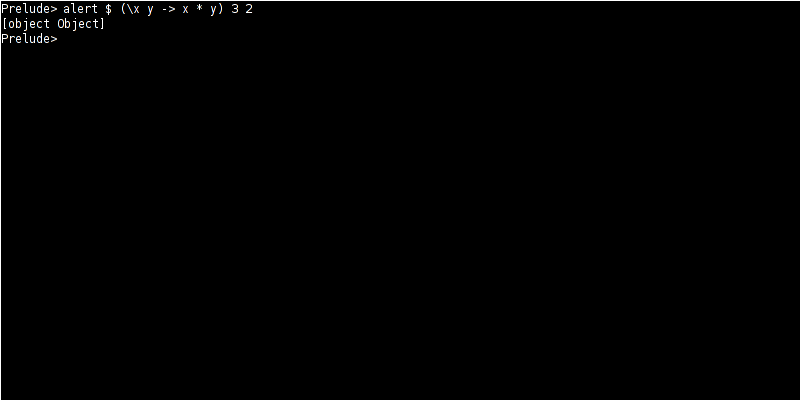
\includegraphics[width=1\textwidth]{hiji_screen3.png}
        \caption{HIJi användargränssnitt}
    \end{center}
\end{figure}

Figur 2 visar hur HIJi ser ut för användaren. De första raderna visar precis som i GHCi vilka moduler som för närvarande är laddade. I detta exemplet är det en modul laddad med namnet Prelude. Därefter följer en prompt där användaren fritt kan skriva in egna funktioner. I figuren visas en lambda-funktion.

%ODO get source from cp-book at home

%HIJi är tänkt att erbjuda användaren liknande möjligheter som GHCi. 

\subsubsection{Fördelar och nackdelar kontra GHCi}
Fördelen med HIJi framför GHCi är att användaren ej behöver ladda ner den stora GHC-kompilatorn på sin personliga dator för att testa enkla Haskelluttryck direkt i webbläsaren. Den åtgångna tiden från viljan att testa Haskell till tidpunkten att man faktiskt sitter med det framför sig kortas. 
Nackdelar gentemot GHCI är att HIJi är en nedbandat version utav GHCi. HIJi kan bara evaluera enklare uttryck. Det finns i dagsläget inga möjligheter att ladda upp hela Haskell-filer för att köra dem. Att som i GHCi på ett enkelt sätt kolla upp  typen av en funktion stöds ej.

% MOOAR


% remove!?
Ett stort problem för alla webbutvecklare idag är att de idag marknadsledande webbläsarna tolkar Javascript på olika sätt. Det har därför kommit fram en rad olika kodbibliotek för att lösa detta problemet. Ett av dessa är JQuery som HIJi använder sig utav för att få ett unisont stöd på alla moderna webbläsare. 
% stop remove

